%TODO: ARREGLAR EJERCICIO 1B
\documentclass{article}
\usepackage[utf8]{inputenc}
\usepackage[spanish]{babel}
\usepackage{graphicx, graphics, float, hyperref}
\usepackage{listings}
\usepackage[a4paper, total={6in, 10in}]{geometry}

\title{SSO Práctica 1 Sesión 3}
\author{Andrés Merlo Trujillo}
\date{}
\hypersetup{
    colorlinks=true,
    linkcolor=black,
}

\begin{document}

\maketitle

%\tableofcontents
%
%\newpage
%\addcontentsline{toc}{section}{Ejercicio 1}
%\section*{Ejercicio 1}
%\begin{figure}[H]
%    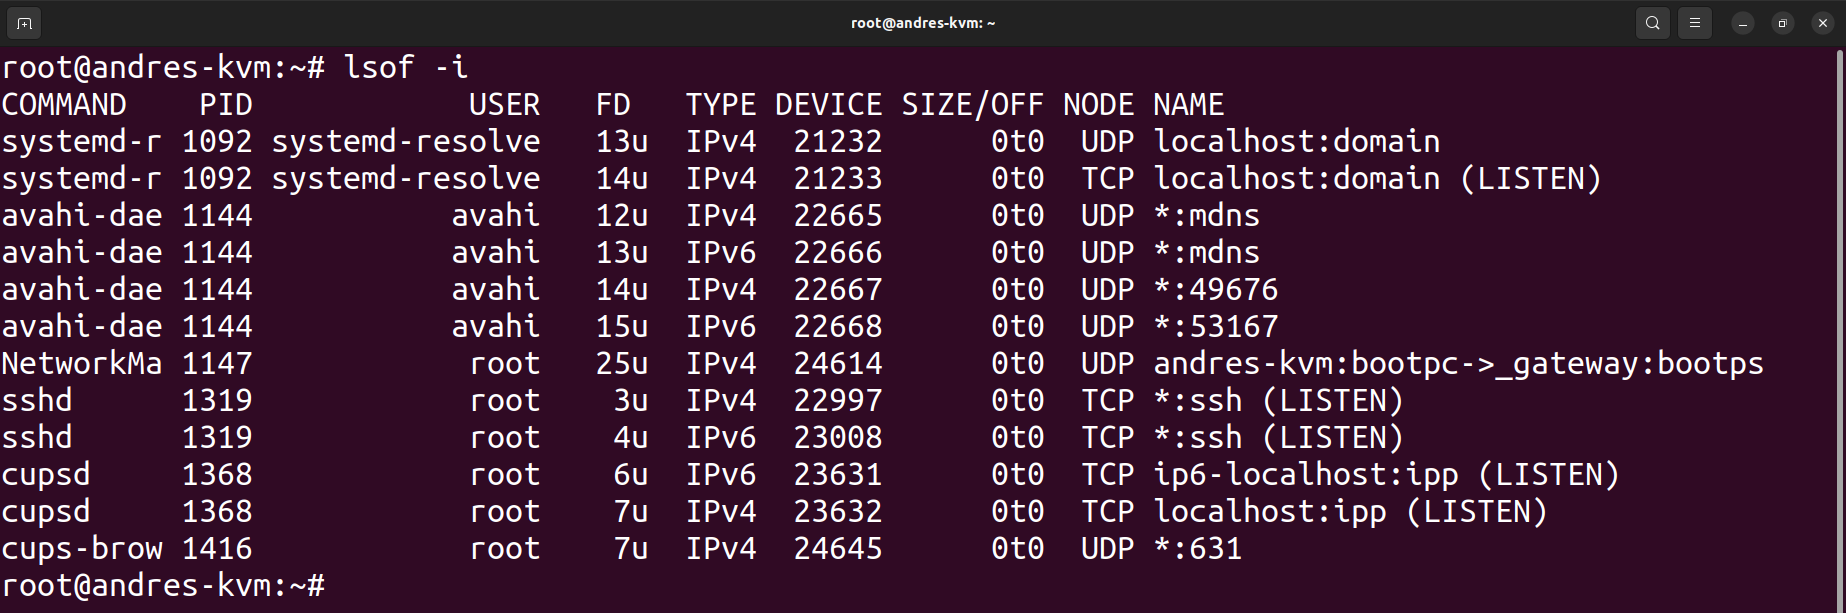
\includegraphics[width=\textwidth]{imagenes/lsofi.png}
%\end{figure}

\addcontentsline{toc}{section}{Ejercicio 1}
\section*{Ejercicio 1}
Con la orden \verb|aa-status| o la orden \verb|apparmor_status| se pueden ver los perfiles activos en Ubuntu:

%foto de los perfiles
%caption: como se puede ver hay 42 perfiles cargados.

Ahora voy a elegir el perfil \verb|/usr/bin/freshclam|, para poder ver el archivo del perfil asociado basta con irse al directorio \verb|/etc/apparmor.d| y el archivo se denomina igual que la ruta absoluta del mismo, pero en vez de usar ``/'' se utilizan puntos. Por tanto, el archivo deseado es: \verb|/etc/apparmor.d/usr.bin.freshclam|.

\begin{figure}[H]
    \centering
    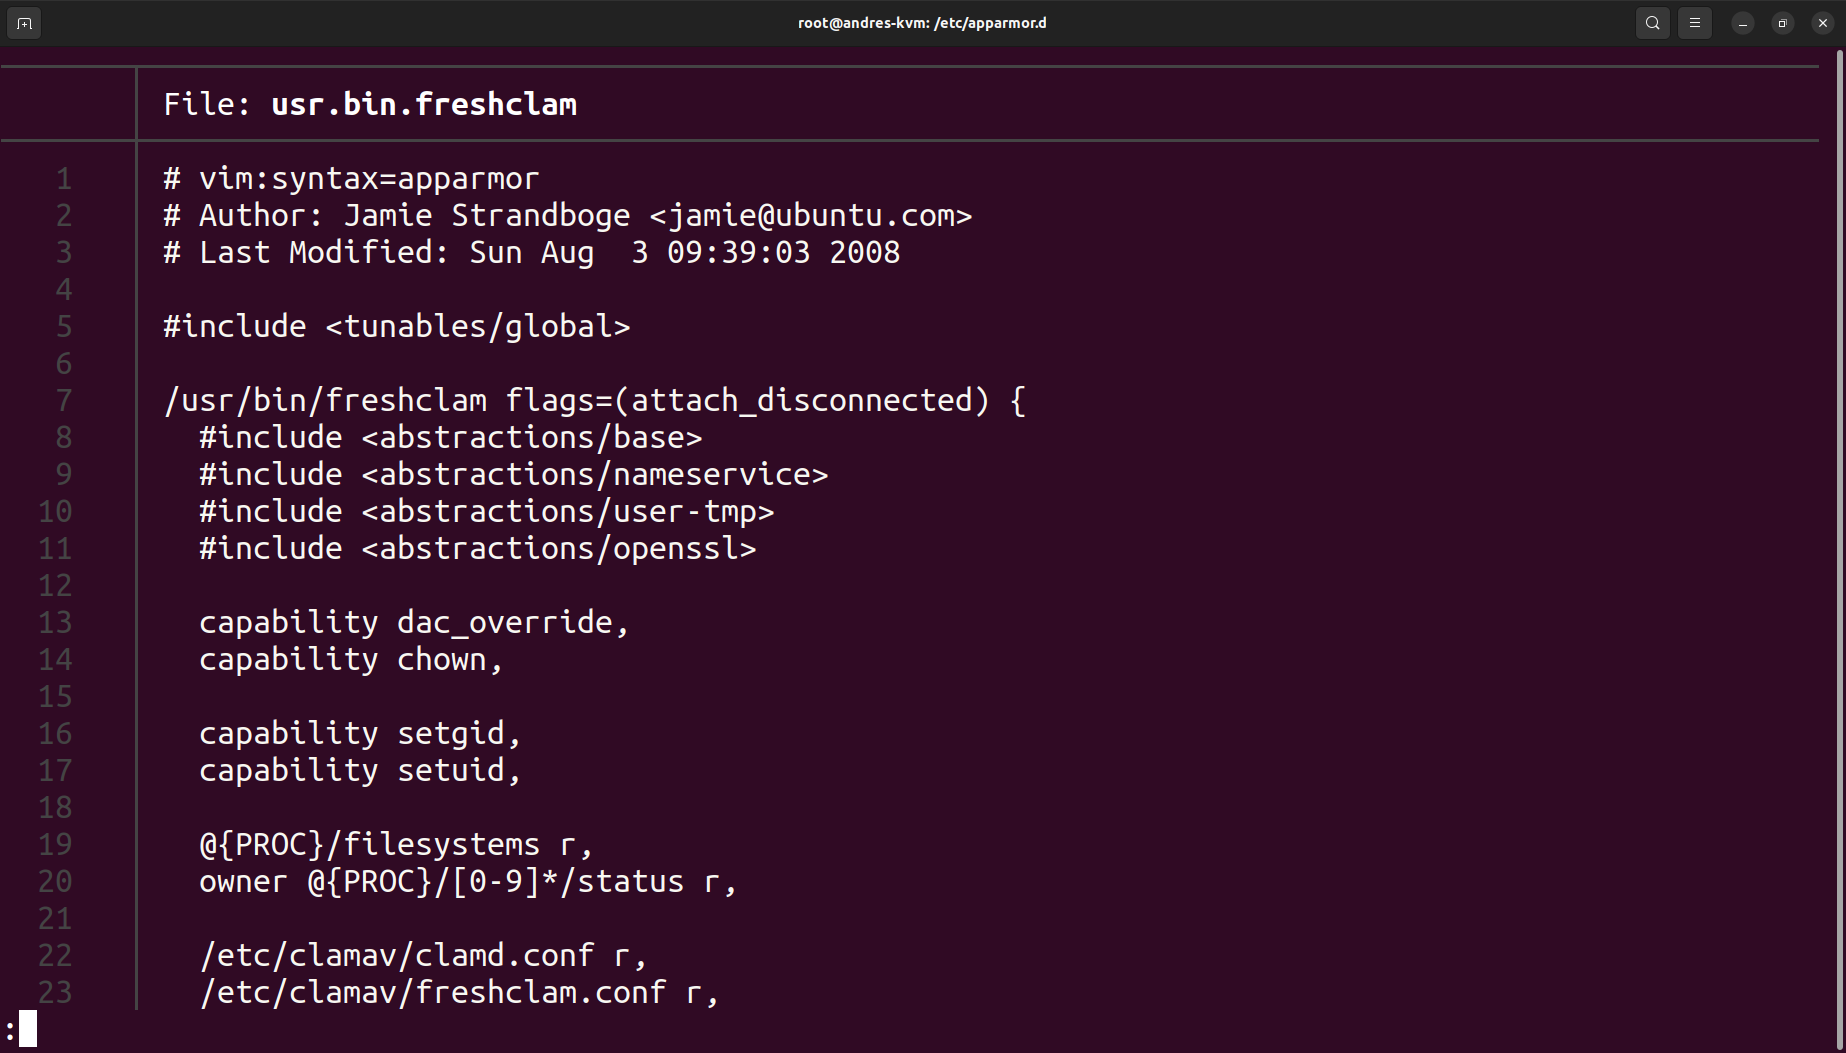
\includegraphics[width=0.85\textwidth]{imagenes/Captura desde 2022-10-18 16-13-59.png}
\end{figure}

\begin{figure}[H]
    \centering
    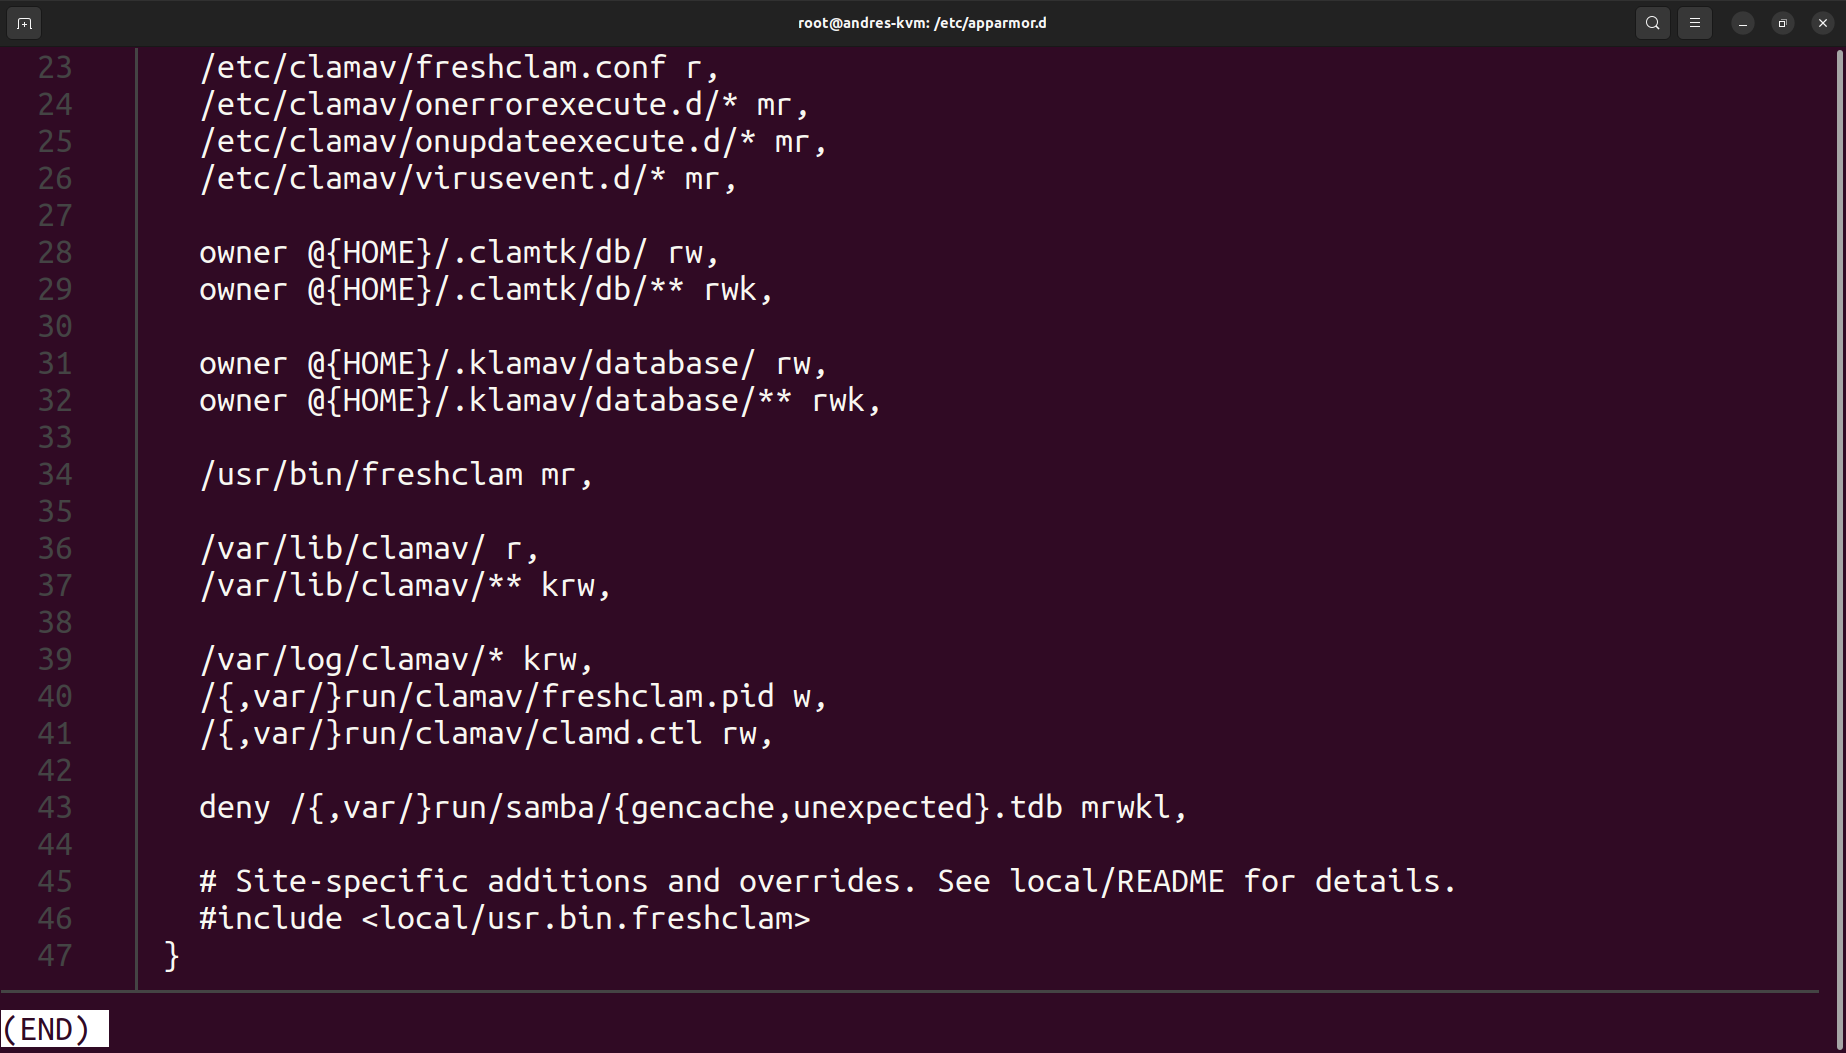
\includegraphics[width=0.85\textwidth]{imagenes/Captura desde 2022-10-18 16-14-08.png}
\end{figure}

\newpage

Las componentes principales son las siguientes:

%https://manpages.debian.org/jessie/apparmor/apparmor.d.5.en.html

\begin{itemize}
    \item \verb|#include <tunables/global>| Carga un archivo que contiene las definiciones de las variables.
    \item \verb|/usr/bin/freshclam| Ruta absoluta del binario.
    \item \verb|#include <abstractions/base>| Obtiene los componentes de los perfiles de AppArmor para simplificar el desarrollo de perfiles.
    \item \verb|#include <abstractions/nameservice>| Incluye las reglas para permitir DNS, LDAP, NIS, SMB, contraseñas de usuarios y grupos, servicios y ``lookups'' de protocolos
    \item \verb|#include <abstractions/user-tmp>| Permite acceder a los directorios temporales
    \item \verb|#include <abstractions/openssl>| Permite acceder a los archivos correspondientes a OpenSSL.
    \item \verb|{,var/}| Permite eliminar líneas innecesarias, poniendo los directorios similares dentro de la lista entre llaves. 
    
    \bigskip

    En este caso las opciones son \verb|/run/clamav/freshclam.pid| y \verb|/var/run/clamav/freshclam.pid|
    %\item \verb|... -> &man_groff| Utiliza el perfil referenciado en la derecha cuando \verb|man| utiliza algun comando de la izquierda.
    %\item \verb|profile ... {| Perfiles secundarios que se ejecutarán cuando estos sean llamados desde el principal. Por ejemplo, mediante el enlace de otro comando desde el perfil principal cuando \verb|freshclam| lo llame.
    %\item \verb|#include <abstractions/console>| Incluye acceso de lectura y escritura a los archivos de dispositivo que controlan las terminales virtuales, sshd, xterm, etc. Es necesario para proogramas que interaccionan con el usuario.
    \item \verb|capability ...| Indica las capabilities que tiene permitidas hacer en el sistema. El listado de todas ellas se puede ver usando \verb|man 7 capabilites|.
    \item \verb|owner archivo| Indica que solo puede acceder al archivo indicado si es el propietario del mismo.
    \item \verb|deny archivo| Deniega el acceso al archivo indicado.
\end{itemize}

Además, aparecen variables del tipo ``@{\dots}''.

El valor de estas variables se almacenan en \verb|/etc/apparmor.d/tunables/file|, donde file es el nombre de la variable.

\begin{figure}[H]
    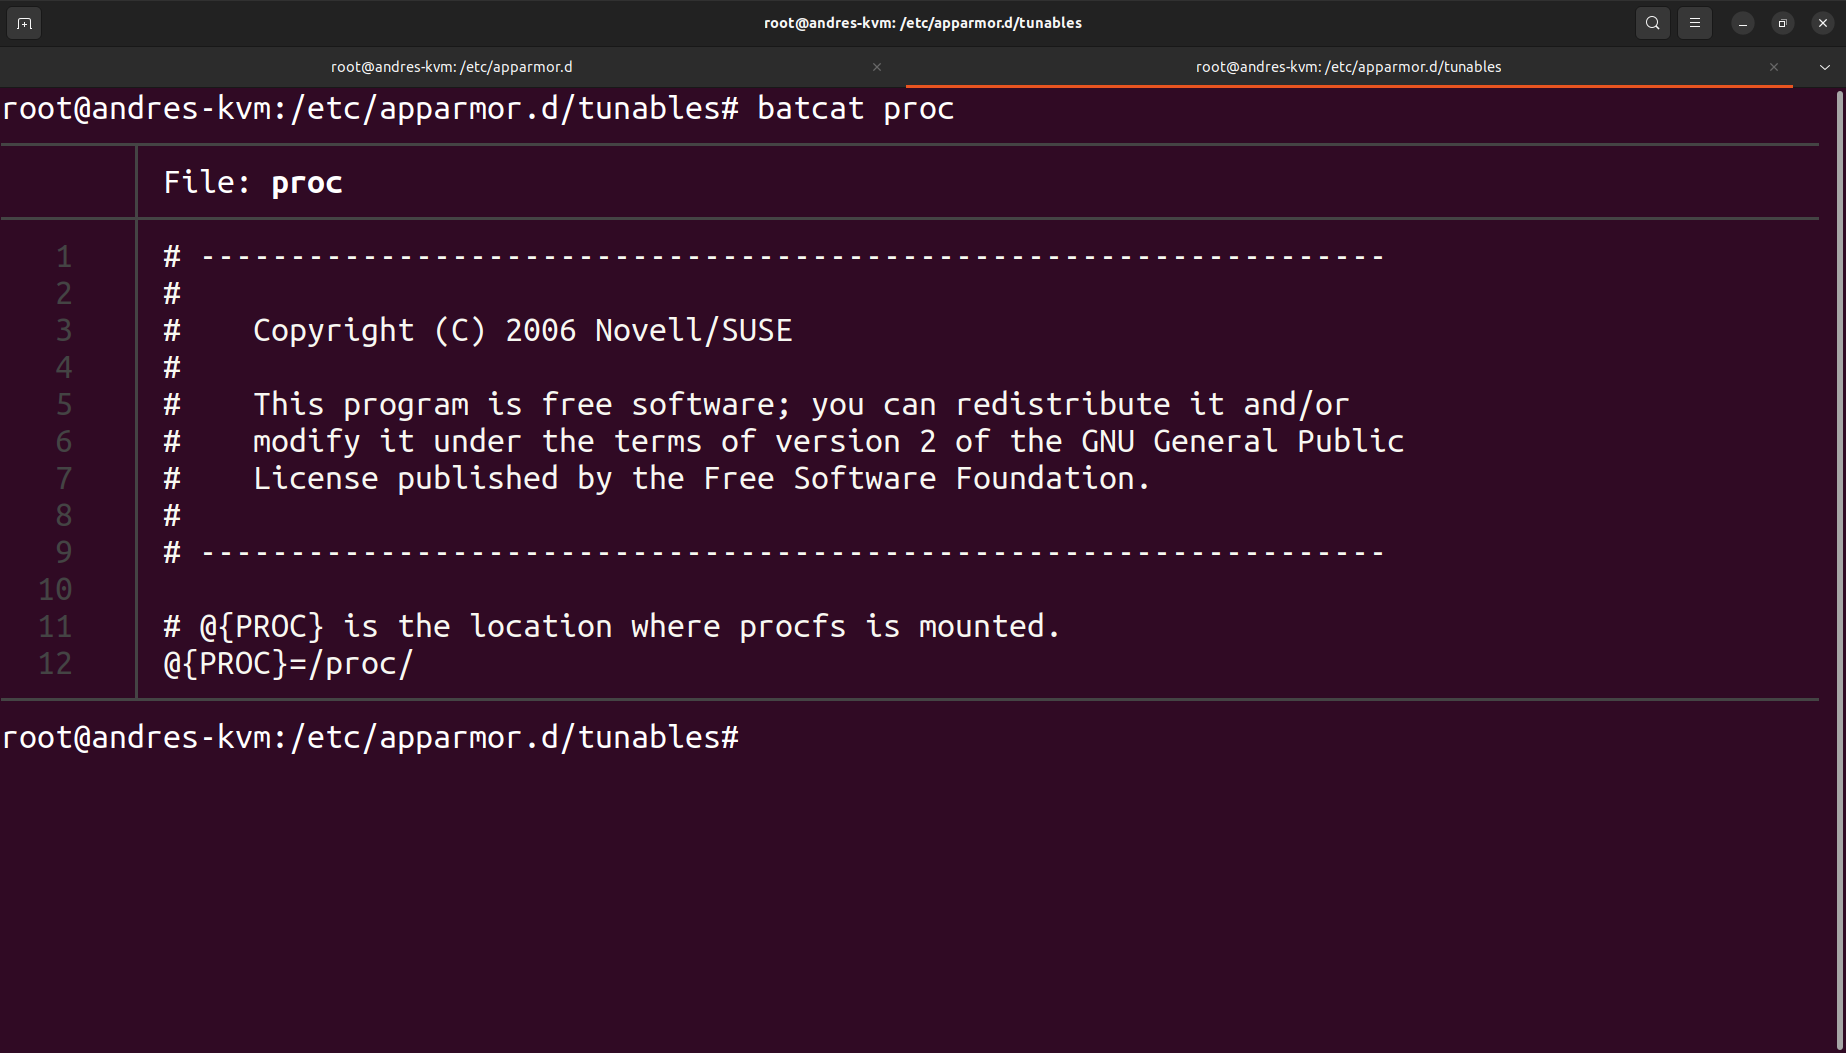
\includegraphics[width=\textwidth]{imagenes/Captura desde 2022-10-18 16-25-52.png}
    \caption{Ejemplo de archivo usado por las variables, en este caso de PROC.}
\end{figure}

\bigskip

Las que aparecen en este perfil son:

\begin{itemize}
    \item \textbf{@\{HOME\}: }Lista de todos los \verb|home| de los usuarios, incluido el root.
    \item \textbf{@\{PROC\}: }Directorio donde procfs es montado.
\end{itemize}

\newpage

También se puede ver que contiene una lista de archivos y directorios junto con sus permisos, estos son los archivos o directorios a los que puede tener acceso, determinado por los switches que se muestran a continuación:

\begin{itemize}
    \item \textbf{r: }Modo lectura.
    \item \textbf{w: }Modo escritura.
    \item \textbf{a: }Modo adjuntar (append).
    \item \textbf{k: }Modo de bloqueo de archivo.
    \item \textbf{l: }Modo de enlace.
    \item \textbf{ux: }Modo de ejecución sin restricciones.
    \item \textbf{Ux: }Modo de ejecución sin restricciones. Además, limpia el entorno (scrub the environment).
    \item \textbf{px: }Ejecución discreta del perfil.
    \item \textbf{Px: }Modo de ejecución discreta del perfil. Además, limpia el entorno (scrub the environment).
    \item \textbf{ix: }Modo de ejecución heredada.
    \item \textbf{m: }Permite \verb|PROT_EXEC| con llamadas a \verb|mmap|.
    \item \textbf{Cx: }Permite transiciones a un perfil hijo. Con la C mayúscula se usa ``secure exec'' de glibc.
\end{itemize}


\addcontentsline{toc}{section}{Ejercicio 2}
\section*{Ejercicio 2}
Voy a generar un perfil para el programa \verb|nano|, la característica principal que voy a añadir es prohibirle el acceso a un archivo denominado \verb|/root/archivoProhibido| el cual contiene lo siguiente:


\begin{figure}[H]
    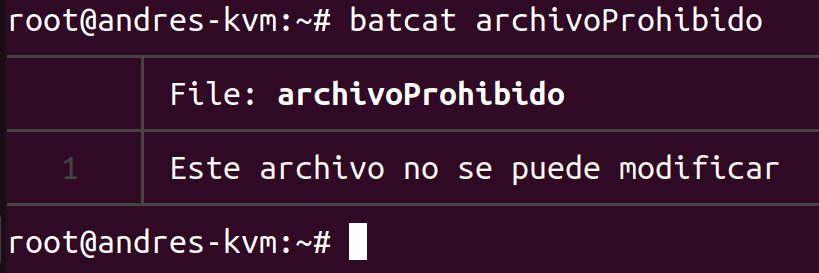
\includegraphics[width=\textwidth]{imagenes/Captura desde 2022-10-18 16-41-05.png}
    \caption{Contenido de ``archivoProhibido''.}
\end{figure}

\bigskip

Para saber su ruta absoluta se puede usar la orden \verb|which nano|:


\begin{figure}[H]
    \centering
    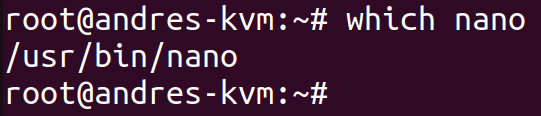
\includegraphics[width=0.6\textwidth]{imagenes/which.png}
\end{figure}

\newpage

Ahora para generar el perfil se ejecuta el comando \verb|aa-genprof /usr/bin/nano|:

%Captura desde 2022-10-18 16-41-31
\begin{figure}[H]
    \centering
    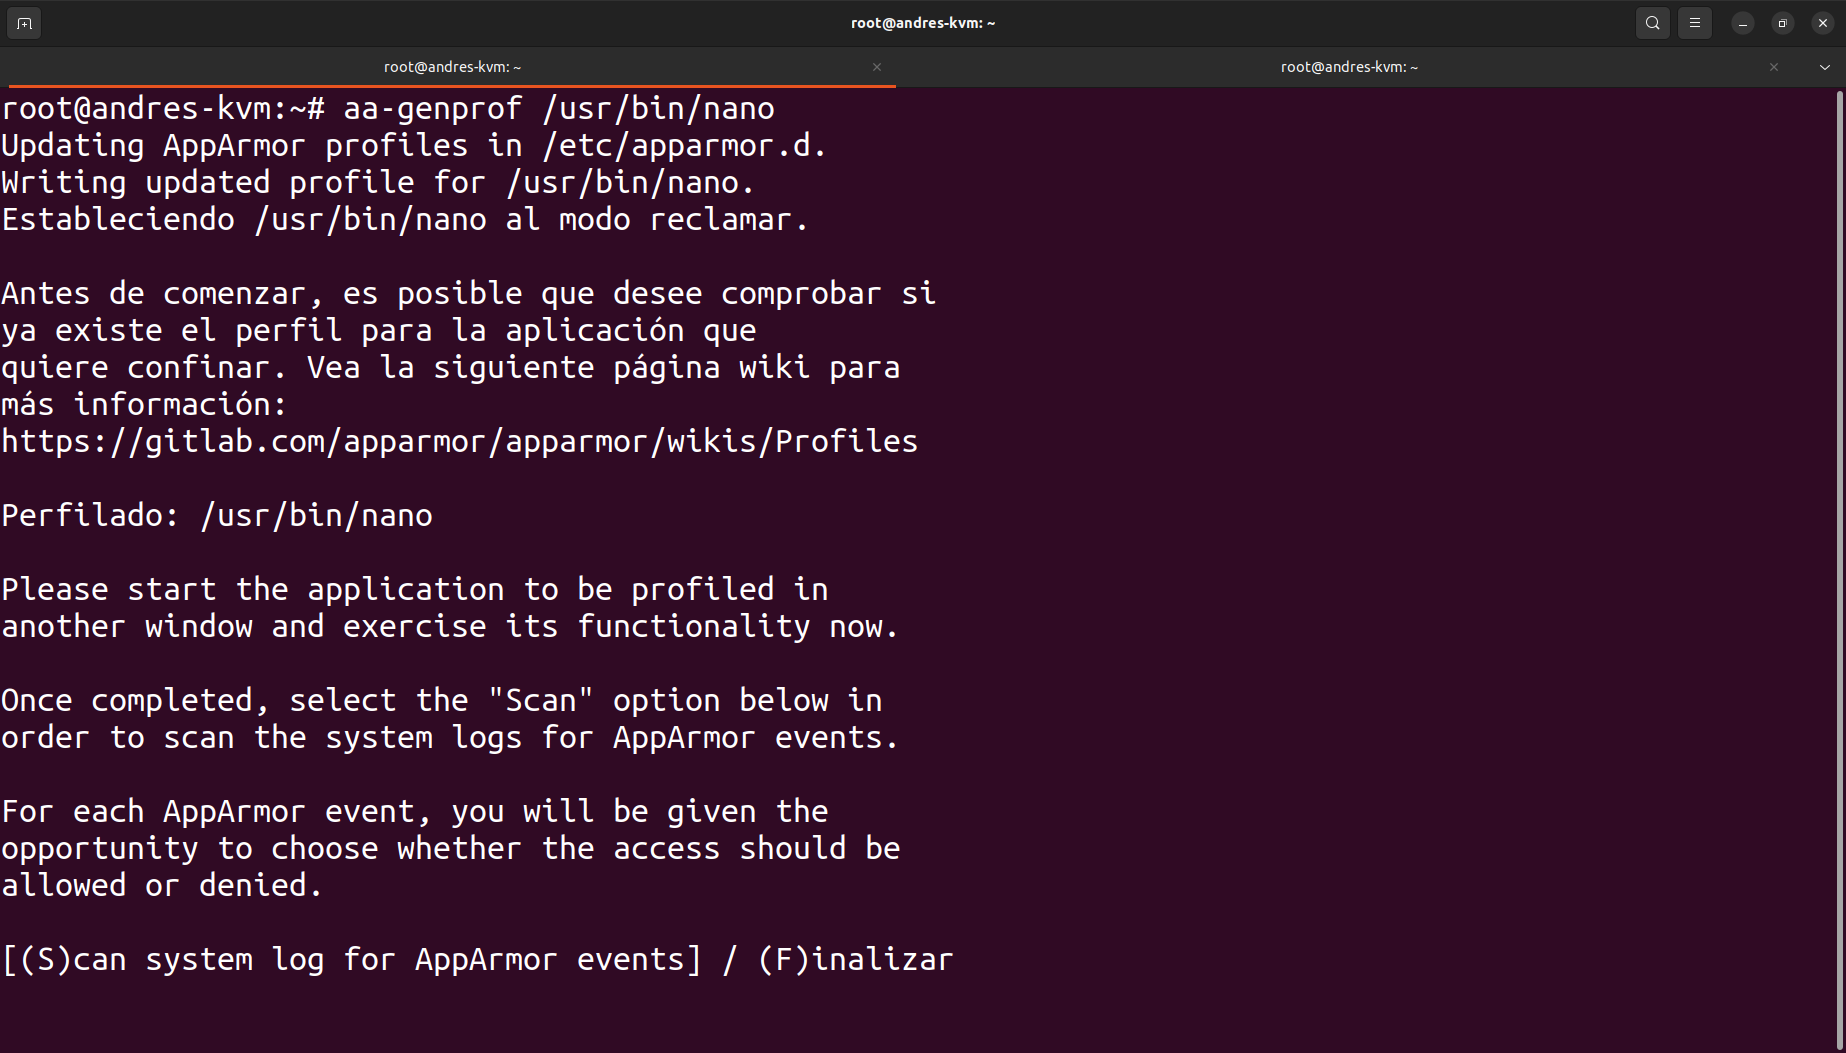
\includegraphics[width=0.6\textwidth]{imagenes/Captura desde 2022-10-18 16-41-31.png}
    \caption{Contenido de ``archivoProhibido''.}
\end{figure}

Ahora pide que abramos el programa a perfilar y pulsemos en el botón de escanear. Abriendo \verb|nano| en otra terminal permitirá continuar con el proceso.

\bigskip

A continuación aparecerán distintos archivos y capabilities relacionadas con las que debemos dar acceso o no.


\begin{figure}[H]
    \centering
    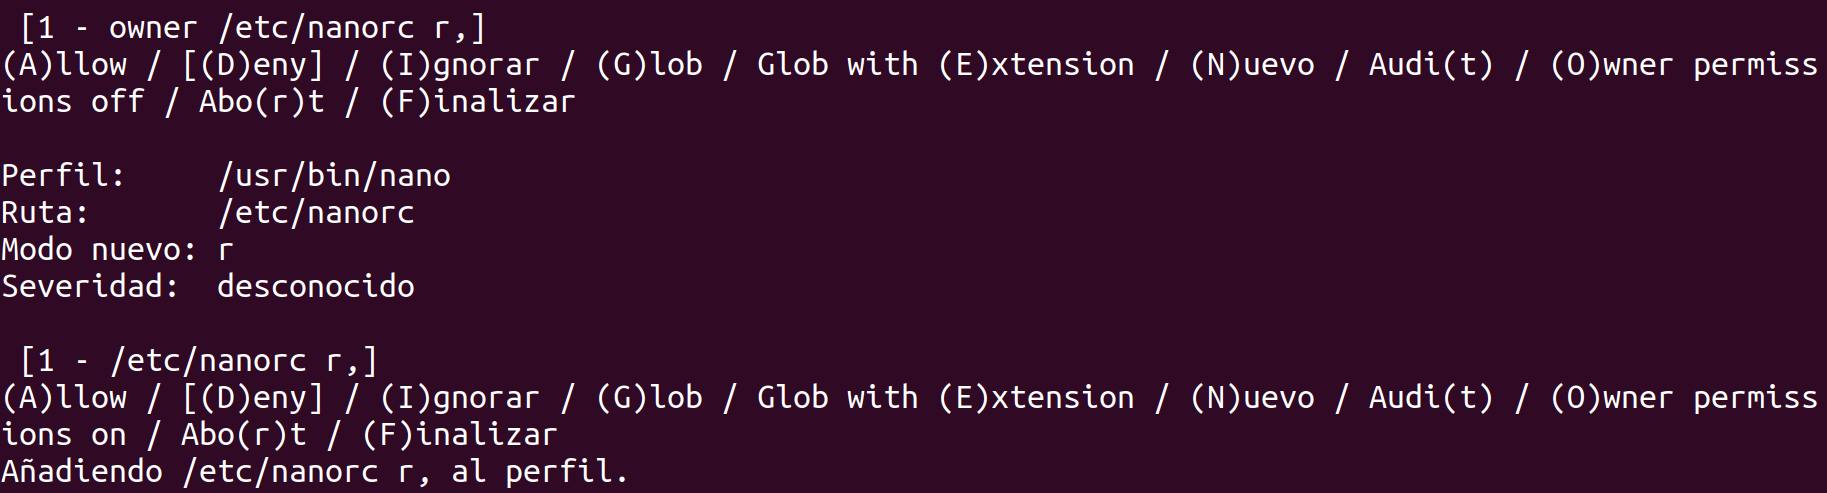
\includegraphics[width=\textwidth]{imagenes/Captura desde 2022-10-18 17-11-50.png}
    \caption{Al pulsar la tecla ``O'' desaparece la palabra ``owner'', permitiendo acceso a todos.}
\end{figure}

Al ser el archivo de configuración de \verb|nano|, es recomendable deshabilitar los permisos de propietario, para que los demás usuarios puedan usarlo y permitirlo.

\bigskip

Además, aparece la opción de denegar el acceso a \verb|/etc/passwd|, tras varias modificaciones he llegado a la conclusión de que es necesario para que detecte los usuarios que no sean root, por lo que hay que ponerle el mismo ajuste que a \verb|/etc/nanorc|.

\newpage

Finalmente, el archivo generado por defecto es el siguiente:
\begin{figure}[H]
    \centering
    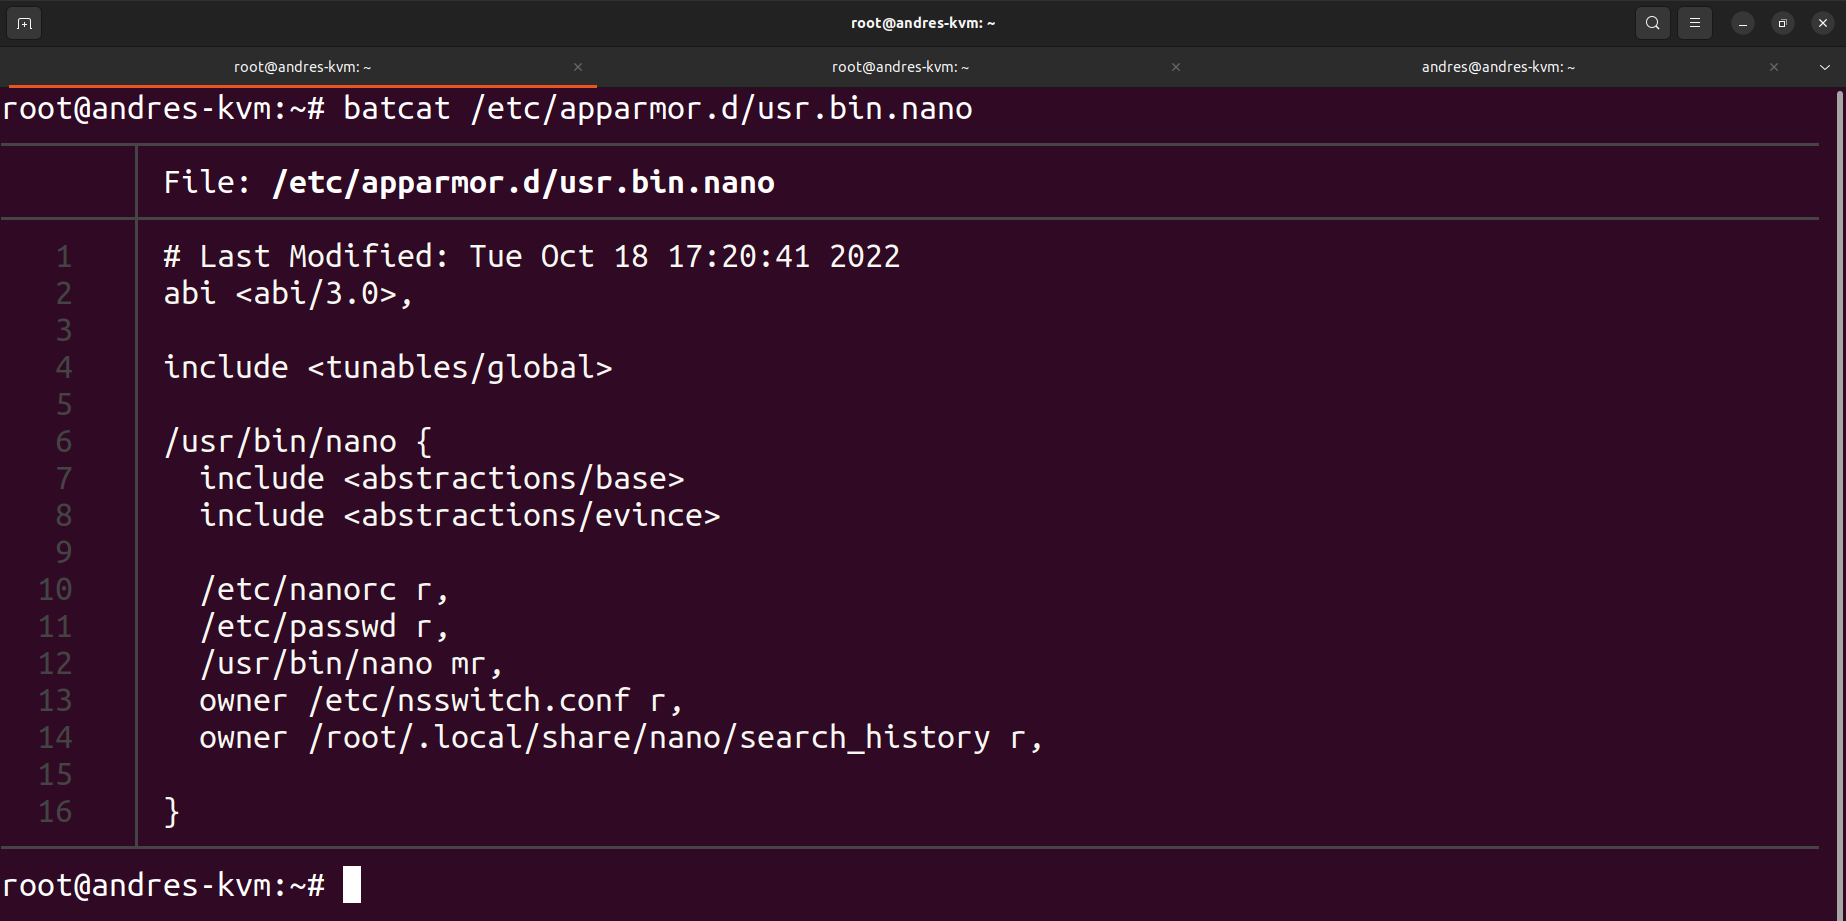
\includegraphics[width=\textwidth]{imagenes/Captura desde 2022-10-18 17-23-45.png}
\end{figure}

Esta configuración va a prohibir por defecto el acceso a todos los directorios, salvo los explícitamente mencionados. Si se quiere que se permita acceso a los directorios \verb|/home| y \verb|/root|, pero prohibiendo el acceso a \verb|/root/archivoProhibido| se debe poner lo siguiente:


\begin{figure}[H]
    \centering
    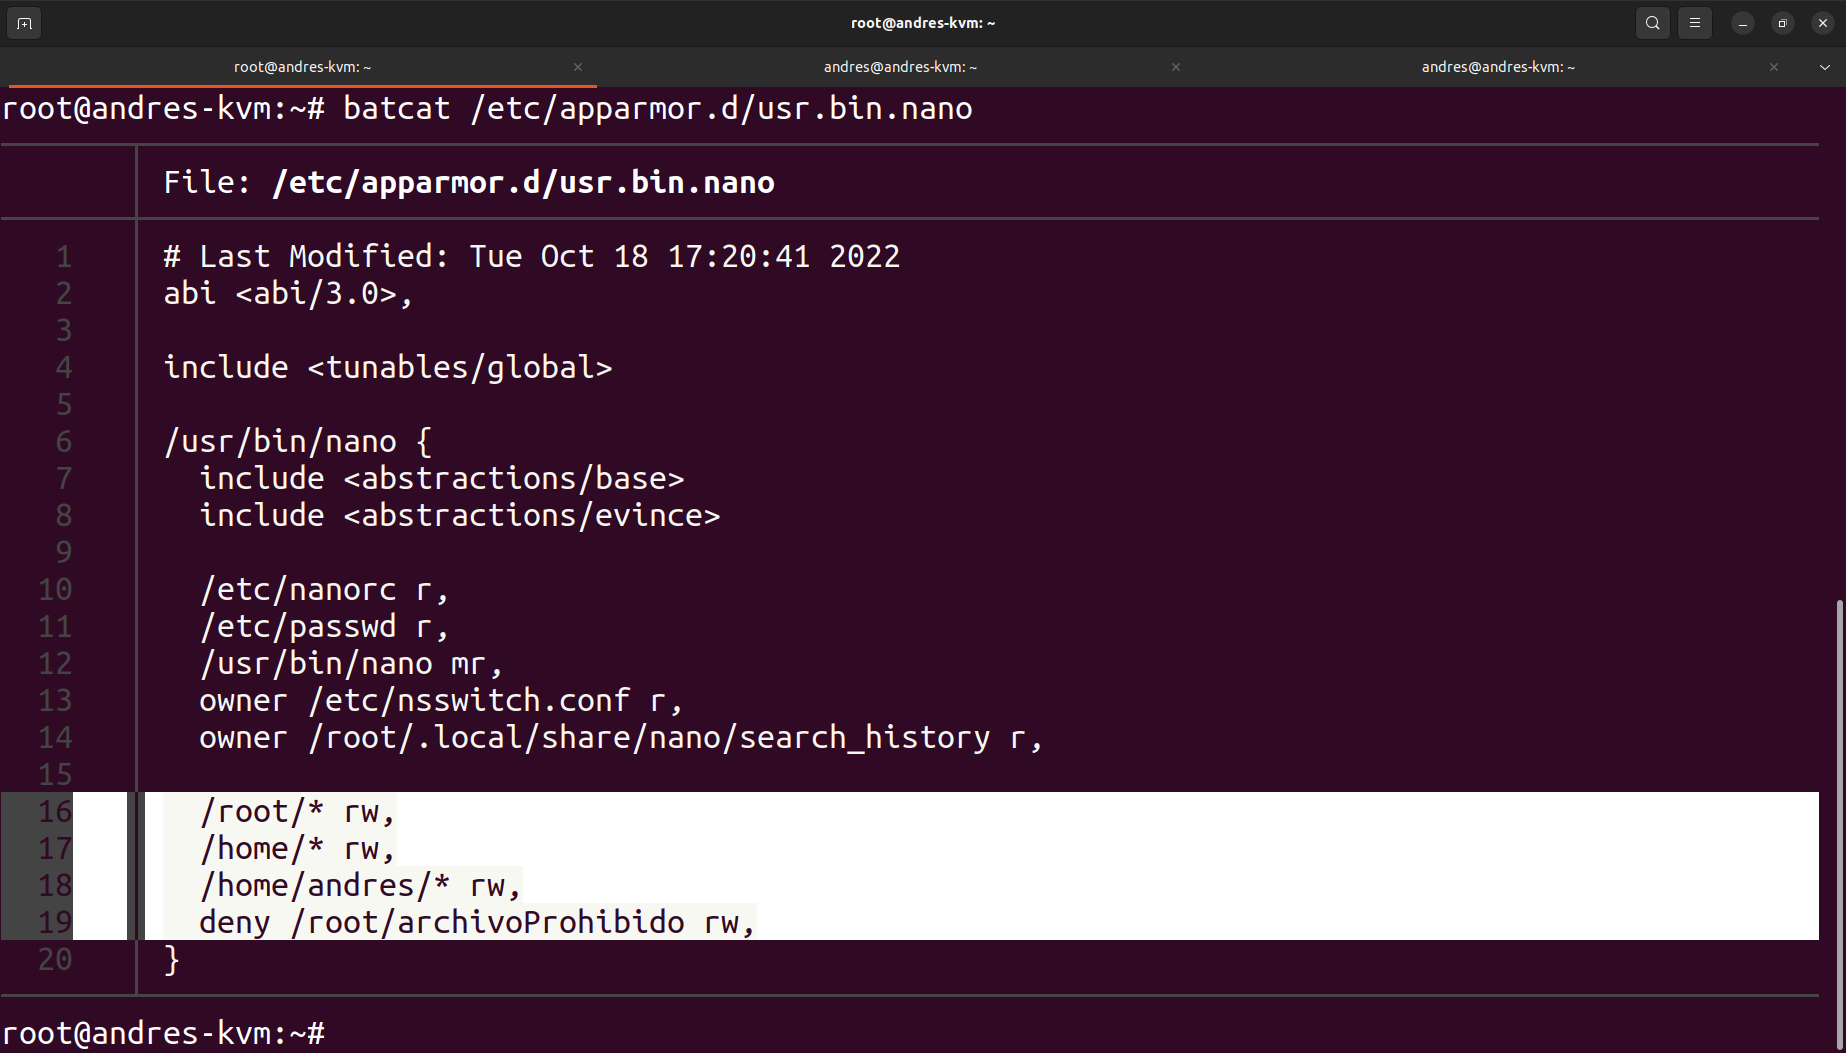
\includegraphics[width=\textwidth]{imagenes/Captura desde 2022-10-18 17-30-04.png}
\end{figure}

Ahora, haciendo \verb|systemctl reload apparmor| se recargan todos los perfiles y como se puede observar, si hago \verb|nano /root/prueba| permite la creación del archivo.

\begin{figure}[H]
    \centering
    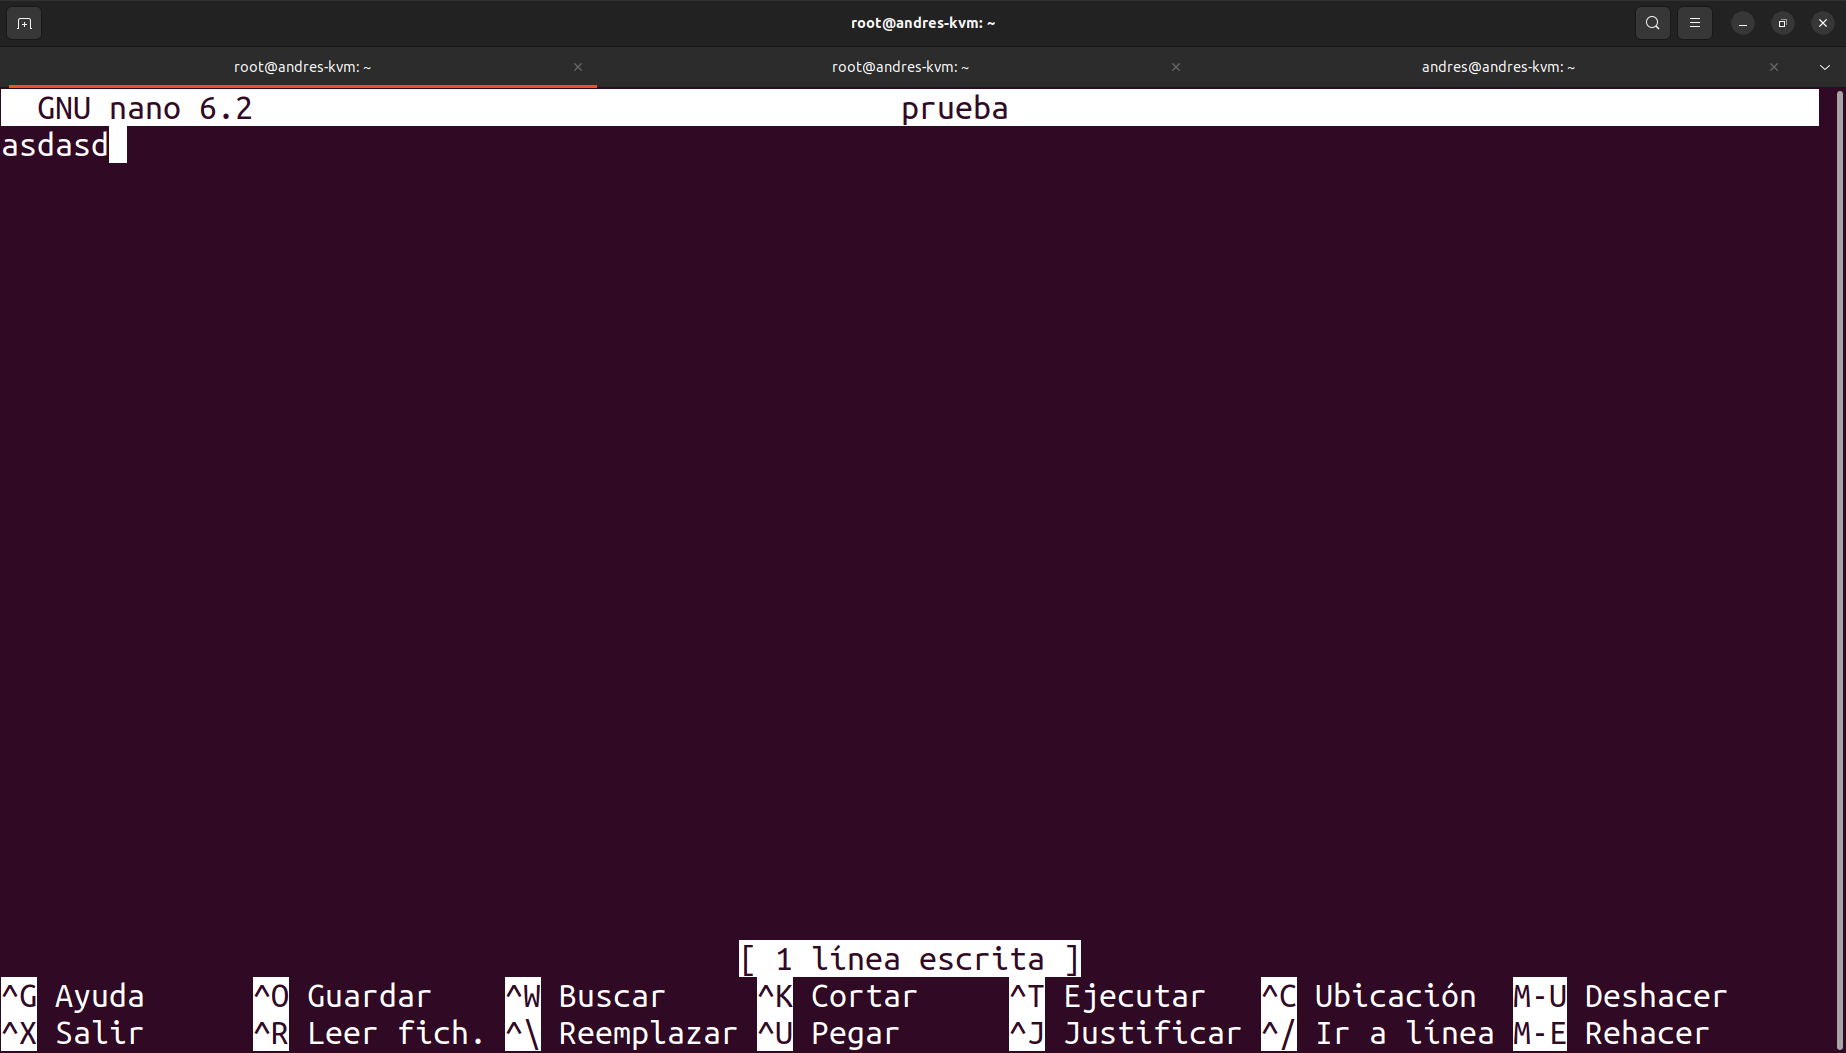
\includegraphics[width=\textwidth]{imagenes/Captura desde 2022-10-18 17-26-43.png}
    \caption{Permite la creación de un archivo en el directorio home de root.}
\end{figure}

\bigskip

Sin embargo, si intento hacer \verb|nano /root/archivoProhibido| no permite ni visualizarlo:

\begin{figure}[H]
    \centering
    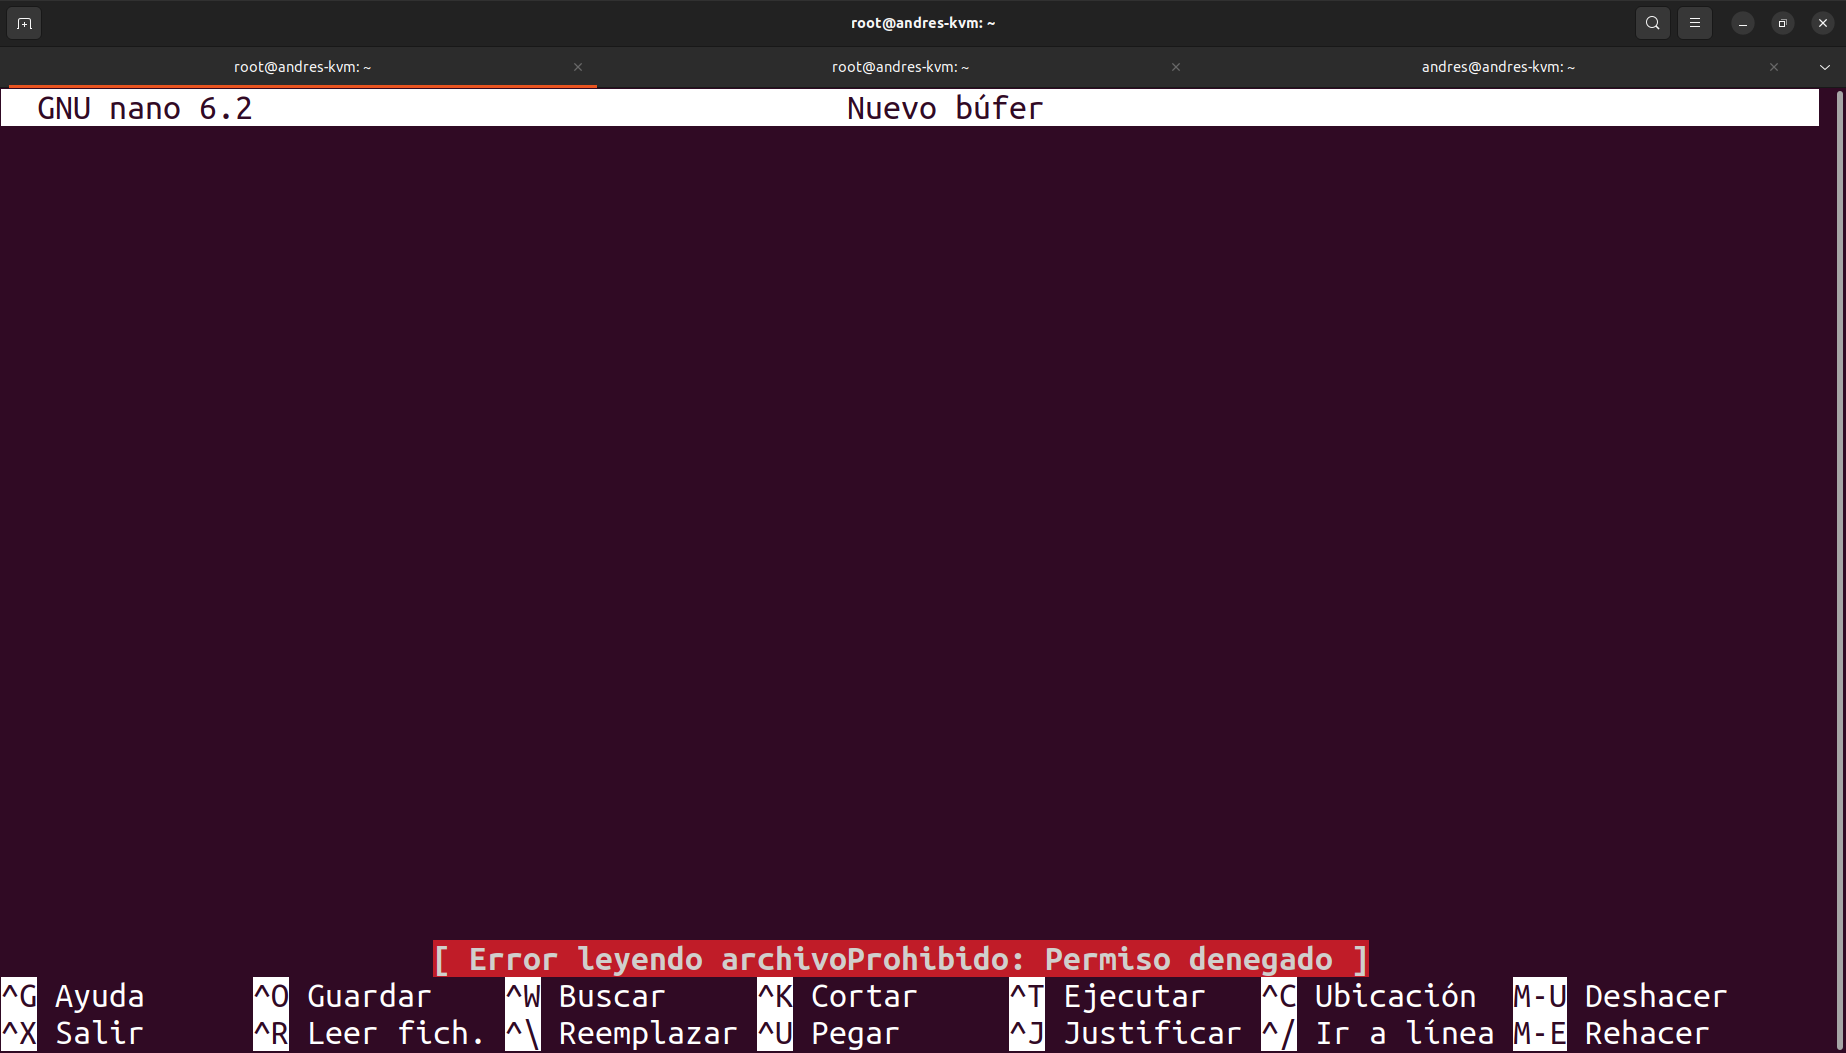
\includegraphics[width=\textwidth]{imagenes/Captura desde 2022-10-18 17-26-52.png}
    \caption{Sigue prohibiendo el acceso a este archivo, ya que está explícitamente prohibido con ``deny''.}
\end{figure}

\end{document}

%\begin{figure}[H]
%    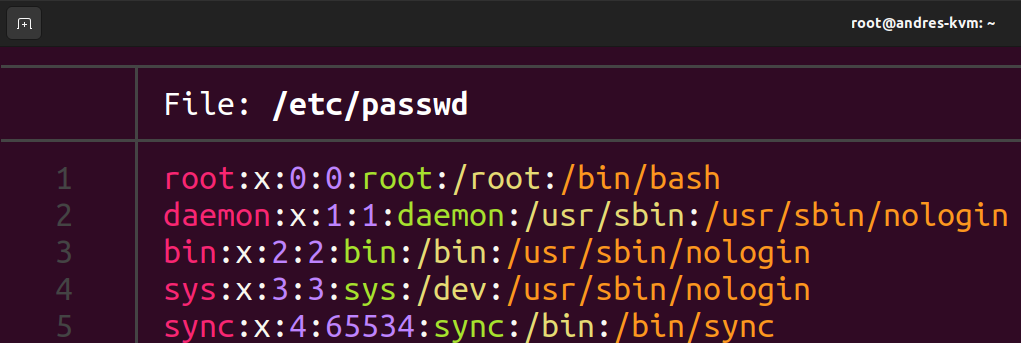
\includegraphics[width=\textwidth]{imagenes/passwdfile.png}
%    \caption{Ejemplo de entradas en el archivo.}
%\end{figure}